\documentclass[14pt]{book}

\usepackage{fancyhdr}
\usepackage{graphicx}
\usepackage[margin=2.5cm]{geometry}
\usepackage{graphicx}
\usepackage{anysize}
\usepackage{xcolor}
\usepackage{caption}
\usepackage{subcaption}

\marginsize{2cm}{2cm}{2cm}{2cm} % Izquierda, derecha, arriba, abajo
\setlength{\parindent}{0cm}
\pagestyle{fancy}
\fancyhf{}
\fancyhead[L]{\footnotesize Redes de computadoras} %encabezado izquierda
\fancyhead[R]{\footnotesize David Pérez Jacome}   % derecha
\fancyfoot[L]{\footnotesize}  %izquierda
\fancyfoot[C]{Página \thepage}
\renewcommand{\footrulewidth}{0.4pt}

\begin{document}
\begin{center}
  \newcommand{\HRule}{\rule{\linewidth}{0.5mm}}
  \begin{minipage}{0.48\textwidth}
    \begin{flushleft}
      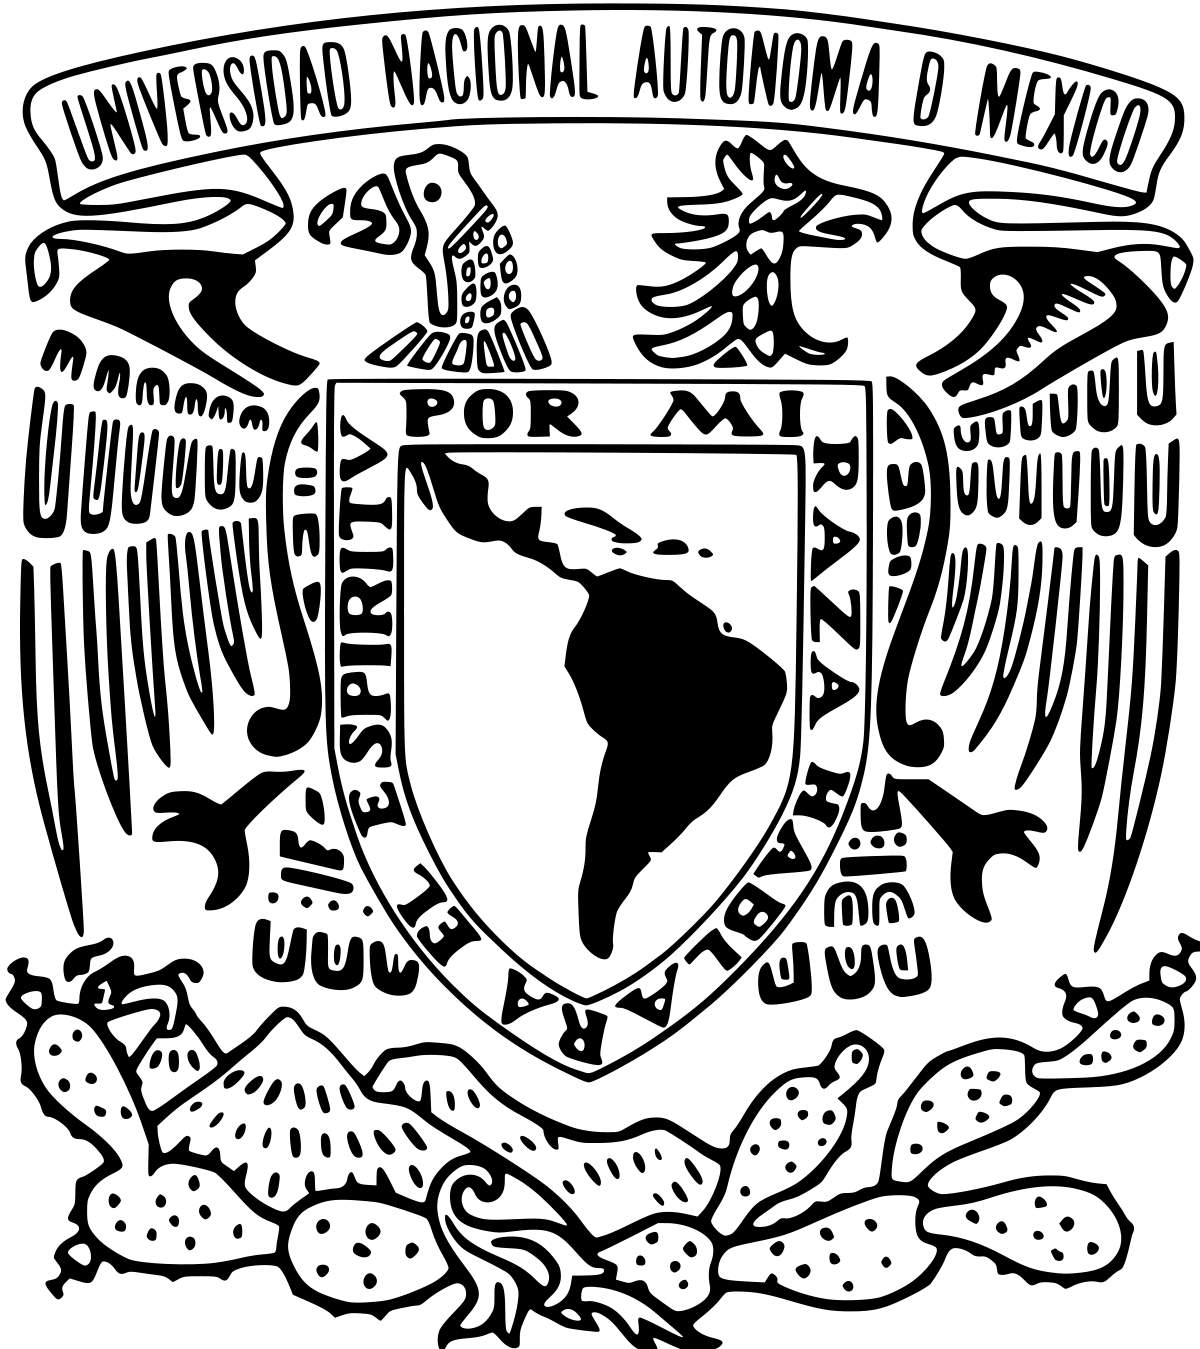
\includegraphics[scale = 0.08]{images/logo_unam.png}
    \end{flushleft}
  \end{minipage}
  \begin{minipage}{0.48\textwidth}
    \begin{flushright}
      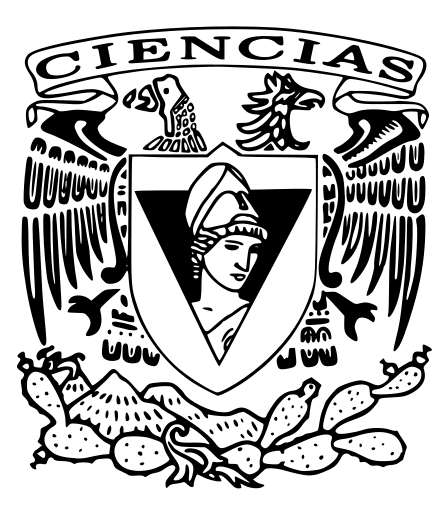
\includegraphics[scale =0.22]{images/logo_ciencias.png}
    \end{flushright}
  \end{minipage}
  \vspace*{-1.5cm}
  \textsc{\huge Nacional Autónoma de México \\ \vspace{-4px} Universidad }\\[2cm]
  \textsc{\LARGE Facultad de Ciencias}\\[1.5cm]
  \begin{minipage}{0.9\textwidth}
    \begin{center}
      \textsc{\LARGE Redes de computadoras}
    \end{center}
  \end{minipage}\\[0.5cm]
  \vspace*{1cm}
  \HRule \\[0.4cm]
  { \huge \bfseries Practica 04}\\[0.4cm]
  \HRule \\[1.5cm]
  \begin{minipage}{0.52\textwidth}
    \begin{flushleft} \large \small \vspace{-0.6cm} \vspace{-0.6cm}
      Alumno David Pérez Jacome \\
    \end{flushleft}
  \end{minipage}
  \begin{minipage}{0.46\textwidth}
    \vspace{-0.6cm}
    \begin{flushright} \large \small \emph{Profesor:}
      Paulo Santiago de Jesús Contreras Flores	 \\
    \end{flushright}
  \end{minipage}
  \vspace*{1cm}
  \vspace{2cm}
  \begin{center}
    {\large 2023}
  \end{center}
\end{center}
\newpage

{\color{blue} \section*{\textbf{Reporte de practica de laboratorio.}}}
\vspace{1em}

{\color{blue} \subsection*{\textbf{Desarrollo.}}}
\vspace{1em}

Es importante recalcar que este es el readme de la practica 04.\\

Para iniciar esta practica tomé como referencia el archivo que nos brindaron en la pagina de git. Con base a esto nos quedo el siguiente archivo:\\

\begin{figure}[h]
  \centering
  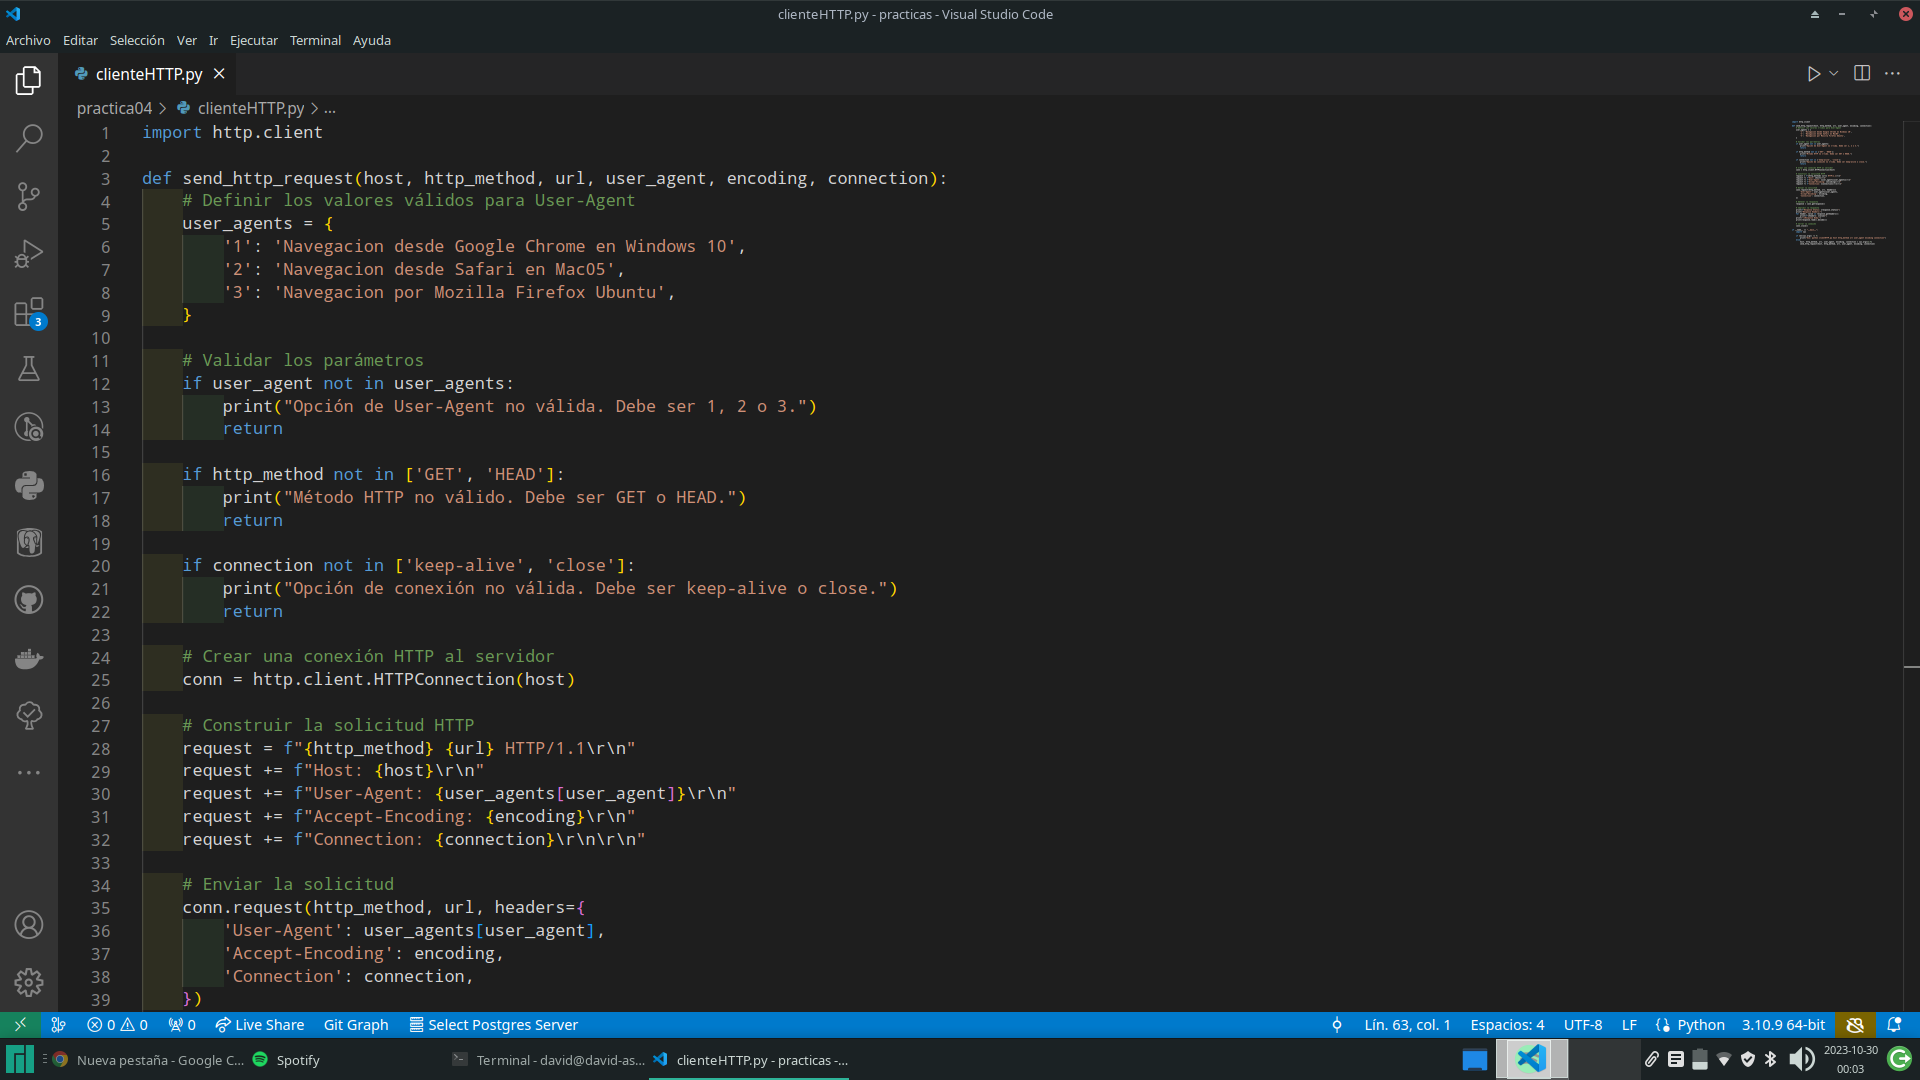
\includegraphics[width=15cm]{images/capturaaaaaaaaaaa.png}
\end{figure}

Despúes de esto probamos nuestro codigo con los parametros seleccionados y entonces probamos que la ejecución es todo un exito:
\textbf{python clienteHTTP.py www.mundonano.unam.mx GET / 1 identity close}\\

\begin{figure}[h]
  \centering
  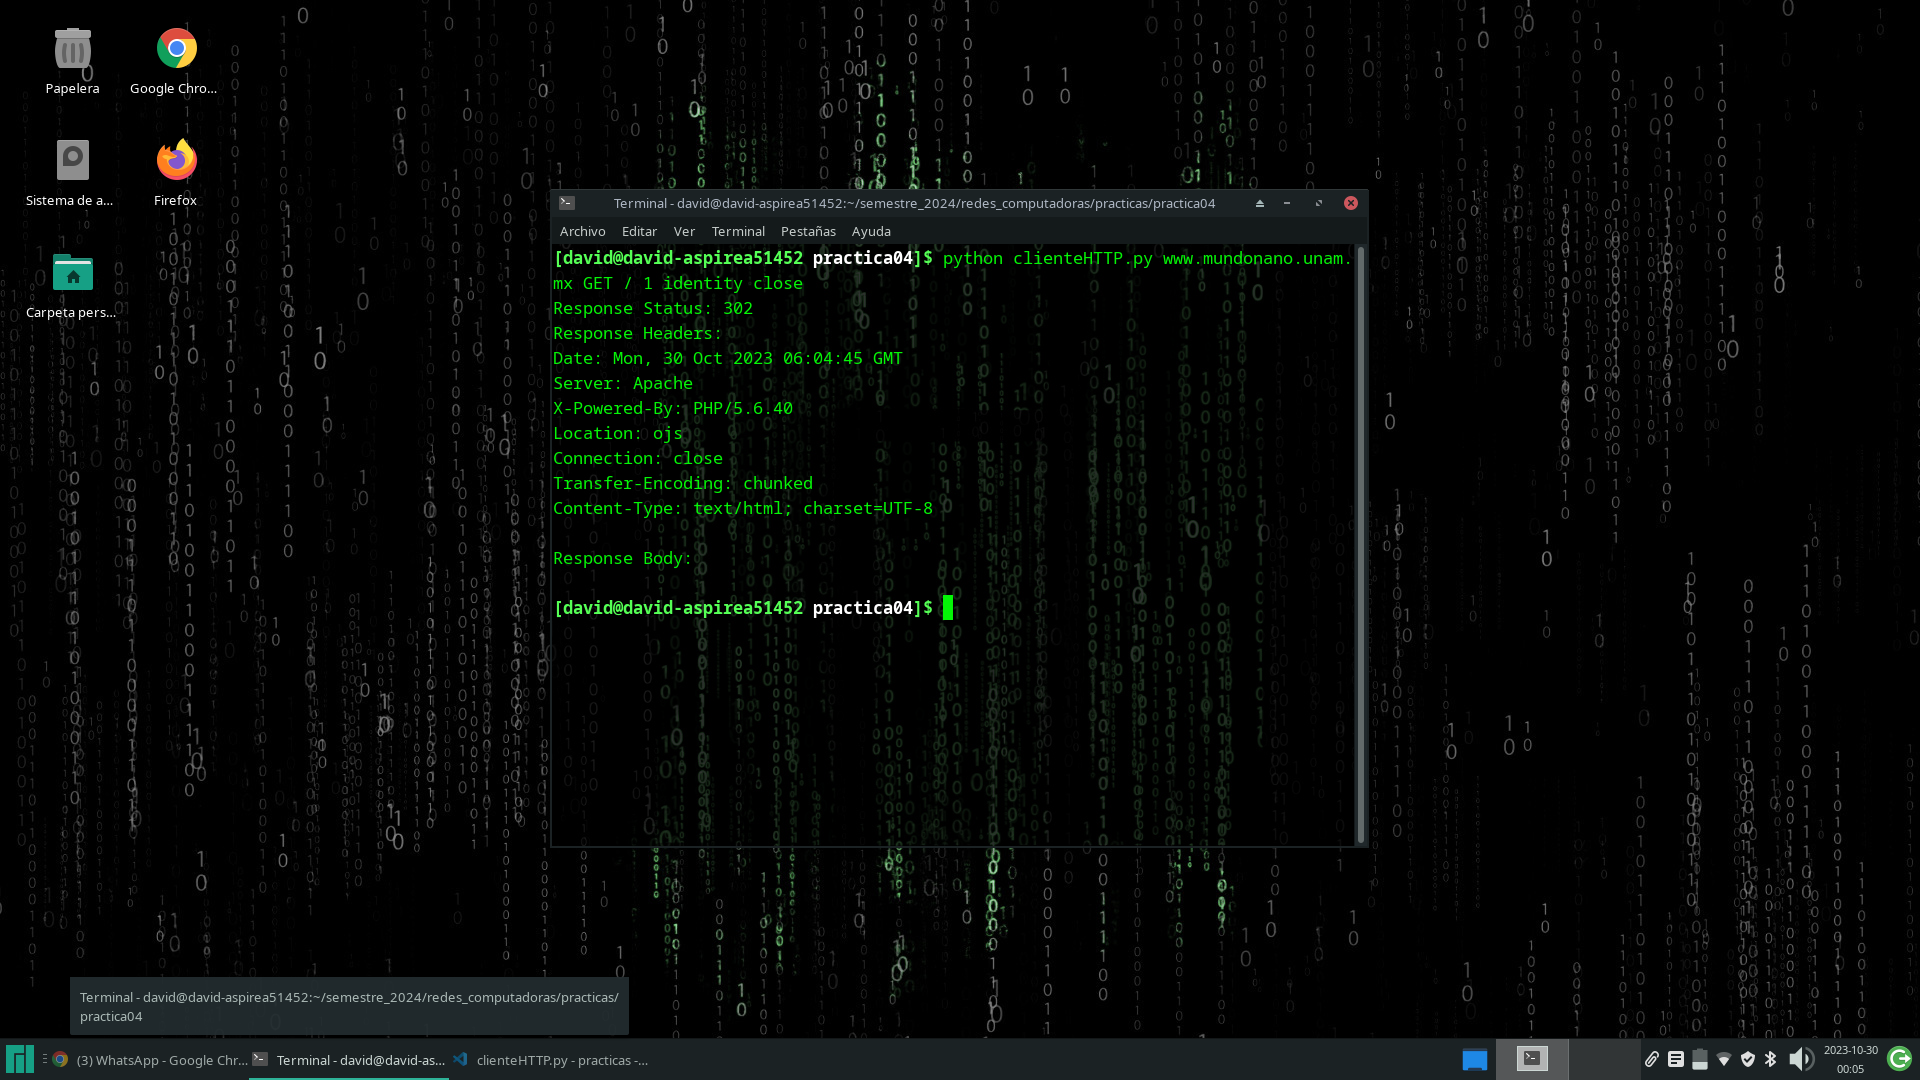
\includegraphics[width=15cm]{images/prueba de jala.png}
\end{figure}

Para la segunda parte de la practica simplemente solo creamos el siguiente archivo con base a nuestro sistema \textbf{ubuntu}\\

\begin{figure}[h]
  \centering
  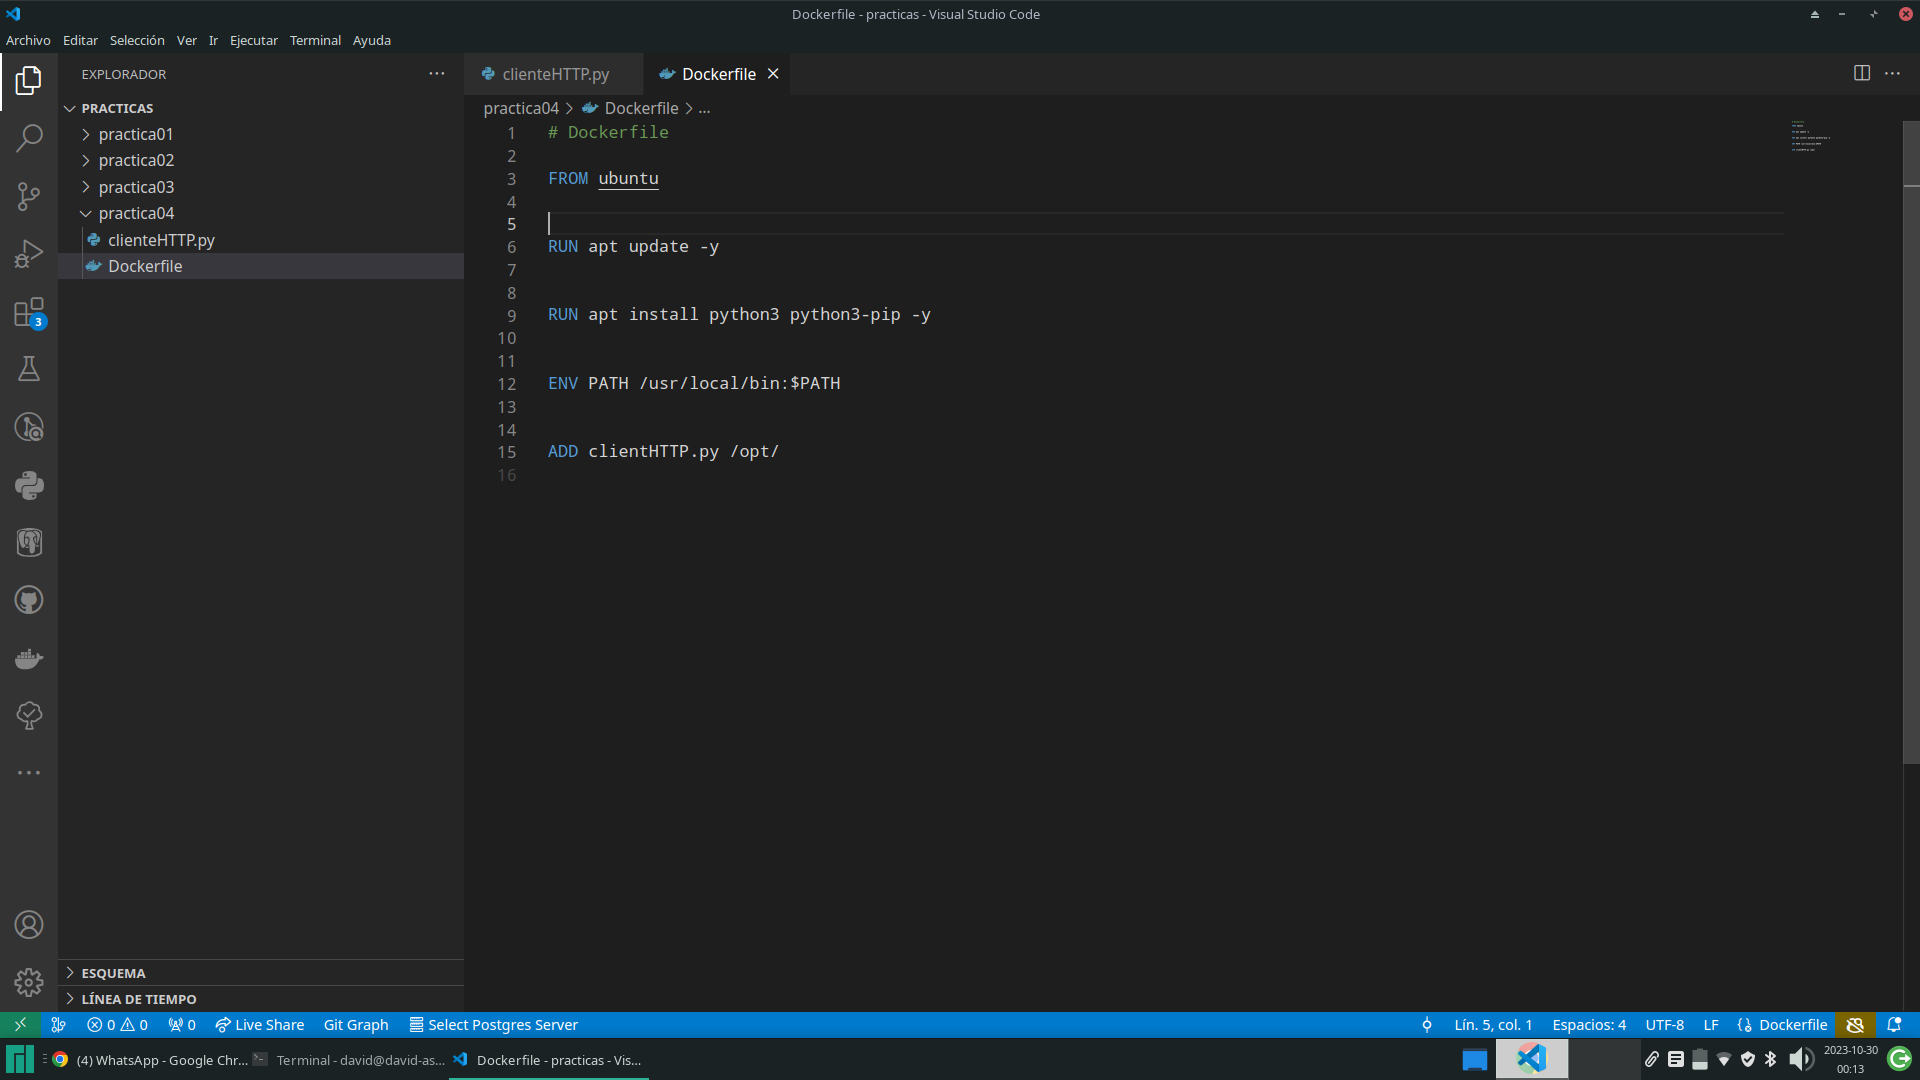
\includegraphics[width=15cm]{images/dockerg.png}
\end{figure}

{\color{blue} \subsection*{\textbf{Preguntas.}}}
\vspace{1em}

\begin{enumerate}
  \item ¿Cuál es la función de los métodos de HTTP HEAD, GET, POST, PUT y DELETE?\\
  \textbf{Los métodos HTTP son utilizados para indicar la acción que se desea realizar sobre un recurso web. A continuación se describen los métodos HTTP más comunes:\\
  \begin{enumerate}
    \item HEAD: Es similar a GET, pero el servidor no devuelve el cuerpo de la respuesta. Se utiliza para obtener información sobre el recurso sin descargarlo.
    \item GET: Se utiliza para obtener un recurso web. El servidor devuelve el cuerpo de la respuesta.
    \item POST: Se utiliza para enviar datos al servidor para su procesamiento. El cuerpo de la solicitud contiene los datos que se envían al servidor.
    \item PUT: Se utiliza para actualizar un recurso web existente. El cuerpo de la solicitud contiene los nuevos datos que se deben almacenar en el servidor.
    \item DELETE: Se utiliza para eliminar un recurso web existente.
  \end{enumerate}}
  \item ¿Investigue y enliste junto con su significado las categorías de códigos de estado que usa HTTP?\\
  \textbf{Los códigos de estado HTTP son utilizados por los servidores web para indicar el resultado de una solicitud HTTP. Los códigos de estado se dividen en cinco categorías:\\
  \begin{enumerate}
    \item Respuestas informativas (100-199): Indican que la solicitud ha sido recibida y que el servidor está procesando la solicitud.
    \item Respuestas satisfactorias (200-299): Indican que la solicitud ha sido recibida, entendida y aceptada por el servidor.
    \item Redirecciones (300-399): Indican que el cliente debe tomar medidas adicionales para completar la solicitud.
    \item Errores del cliente (400-499): Indican que la solicitud contenía información incorrecta o no pudo ser procesada por el servidor.
    \item Errores del servidor (500-599): Indican que el servidor encontró un error al procesar la solicitud.
  \end{enumerate}}
  \item ¿Para qué se usan los campos encoding y connection?\\
  \textbf{Los campos encoding y connection se utilizan en las solicitudes HTTP para especificar cómo se deben codificar los datos de respuesta y cómo se debe establecer la conexión con el servidor, respectivamente. El campo encoding especifica qué algoritmo de compresión se debe utilizar para comprimir los datos de respuesta, mientras que el campo connection especifica si se debe mantener abierta o cerrar la conexión después de que se haya completado la solicitud.}
\end{enumerate}


\end{document}